%        File: courier-problem.tex
%     Created: Fri Oct 23 09:00 PM 2015 C
% Last Change: Fri Oct 23 09:00 PM 2015 C
%
\documentclass{standalone}

\usepackage{tikz}
\usetikzlibrary{positioning, shapes, calc, backgrounds, fit}

\begin{document}
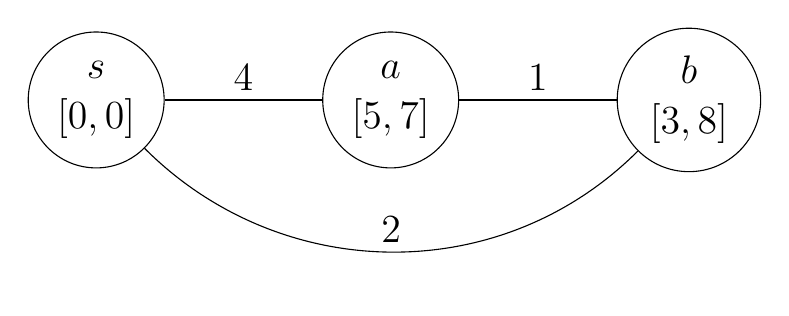
\begin{tikzpicture}[font = \Large, node distance = 2cm, place/.style = {draw, circle, align = 
  center}]
  \node (s) [place] {$s$ \\ $[0,0]$};
  \node (a) [right = of s, place] {$a$ \\ $[5,7]$};
  \node (b) [right = of a, place] {$b$ \\ $[3,8]$};

  \draw[-] (s) to node [above] {$4$} (a);
  \draw[-] (a) to node [above] {$1$} (b);
  \draw[-] (s) to [out = -45, in = -135] node [above] {$2$} (b);
\end{tikzpicture}
\end{document}


